\chapter{Background} \label{chapter:background}

\begin{figure}[!tbp]
	\centering
	\begin{minipage}[t]{0.45\textwidth}
		\centering
    	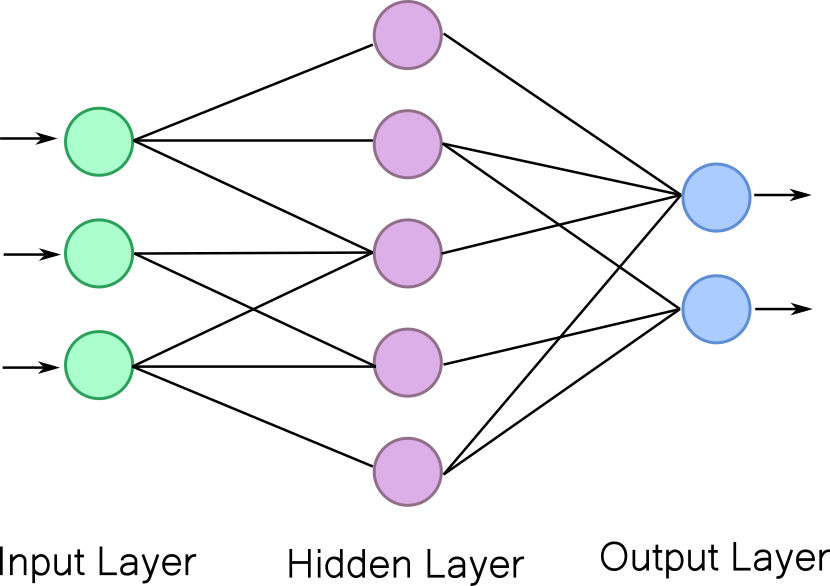
\includegraphics[width=0.6\linewidth]{ffnn}
    	\caption{Abstract structure of a feed-forward neural network. A real network will have many more layers and a lot more neurons per layer. Own figure.}
    	\label{fig:ffnn}
    \end{minipage}
	\hfill
	\begin{minipage}[t]{0.45\textwidth}
		\centering
		\begin{tikzpicture}[scale=0.5, transform shape]
  			\begin{axis}[scale only axis,
    					axis lines=middle,
    					inner axis line style={=>},
    					xlabel={},
    					ylabel={},
    					ytick={-1,-0.5,...,1},
    					xtick={-1,-0.5,...,1},
    					ymin=-1,
    					ymax=1,
    					xmin=-1,
    					xmax=1
  						] 
    			\addplot [mark=none,  blue,   ultra thick] {max(0, x)}; 
  			\end{axis}
		\end{tikzpicture}
    	\caption{Visualization of the ReLU activation function. Own figure.}
    	\label{fig:relu}
    \end{minipage}
\end{figure} 

\section{Neural Networks}

In the last couple of years neural networks and especially deep learning have gained more and more interest. The following sections dissect the individual components of a neural network and explain concepts and procedures.

\subsection{Neuron}

A \textit{Neuron} is the smallest unit of a neural network and is essentially what the network is made up of. It computes the linear function 

\begin{align}
y = \sum\limits_{i=0}^kw_ix_i + b
\end{align}

where $w_i$ is the weight for the $i$-th input $x_i$ and $b$ is a bias. The weights and the bias are the values that can be learned during the training process of the network (see section \ref{section:network_training}). The output of a layer of neurons of a network is the vector $(y_0, \cdots, y_t)$, $y_j$ being the output of the $j$-th neuron. Those outputs then serve as inputs to the next layer, although not every output has to be used by every next neuron. To prevent the network from collapsing into a single linear classifier and thus to increase the expressivity of the network, the output of a neuron is put into a non-linear so-called activation function. Although many different activation functions exist, most popular is the one called \textit{Rectified Linear Unit (ReLU)}, which was first presented by Jarrett et al. in \cite{relu}. The function is exemplarily visualized in fig. \ref{fig:relu} and is calculated as

\begin{align}
f(x) = max(0, x)
\end{align} 

\subsection{Feed-Forward Neural Network}

A \textit{Feed-Forward Neural Network} is a network consisting of layers of neurons. The first layer is called the input layer. Those are the neurons that receive the data that the network is supposed to process. The last layer is called the output layer. The output of the neural network depends on the design implied by the use case. It can be object coordinates like in our case, class probabilities in classification tasks or any other real-valued output. The intermediate layers are called hidden layers. Their number can grow to over a hundred in modern networks \cite{resnet}, thus the name deep neural networks and deep learning. All layers can have different numbers of neurons and connections to previous layers. A schematic overview over the structure of a neural network can be seen in fig. \ref{fig:ffnn}. A neural network can be seen as the function $y=f(x,\theta)$, where $\theta$ are the weights and biases of the neurons and some other parameters an $y$ is the output of the network.

\subsection{Convolutional Neural Networks}

\begin{figure}[!tbp]
	\centering
	\begin{subfigure}[t]{0.45\textwidth}
		\centering
    	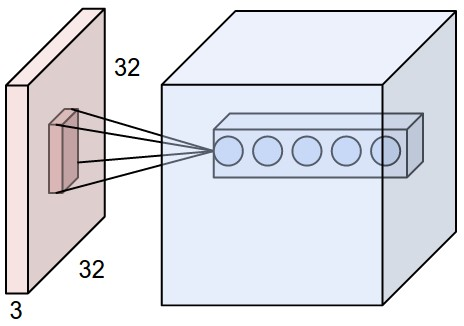
\includegraphics[width=0.7\linewidth]{conv_layer}
    	\caption{Example convolutional layer. The input image has dimensions 32x32 and 3 channels. The blue volume is the actual convolutional layer with multiple filters.}
    	\label{fig:conv_layer}
	\end{subfigure}
	\hfill
	\begin{subfigure}[t]{0.5\textwidth}
		\centering
    	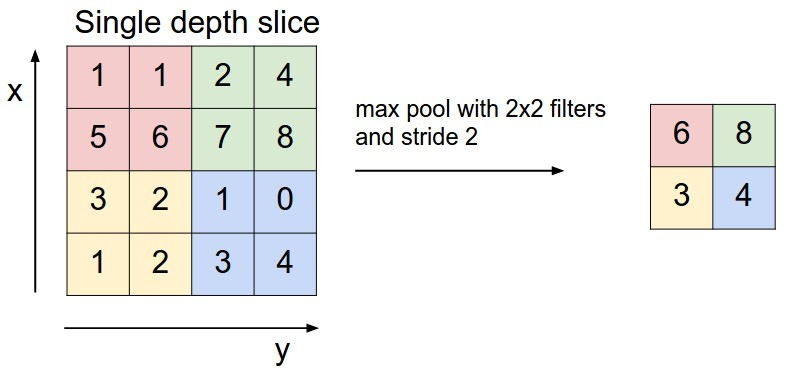
\includegraphics[width=0.9\linewidth]{pool_layer}
    	\caption{Example pooling layer with maximum as pooling operation.}
    	\label{fig:pool_layer}
	\end{subfigure}
	\caption{The two main layer types of a convolutional neural network.}
\end{figure} 

A \textit{Convolutional Neural Network} describes a certain type of feed-forward neural network that consists of mainly two types of layers: \textit{Convolutional Layers} and \textit{Pooling Layers}. Normally, one or more convolutional layers are followed by a pooling layer. A convolutional layer convolves its input with a kernel which is moved along the input's dimensions. The kernel weights are shared, i.e. stay the same for the convolution of the whole input. Fig. \ref{fig:conv_layer} shows the schematic of a convolutional layer. Each filter of the layer extends the output in the third dimension and has its own kernel. To reduce the size of the data a pooling layer can be added after the convolutional layer. This significantly speeds up computation and reduces the memory needed. It also reduces the number of parameters which helps to prevent the network from overfitting. An overfitted network performs well on the data it was trained on but does not generalize well, thus does not perform well on unseen data. Some architectures draw on a \textit{Fully-Connected Layer} as the last layer to perform the actual classification, etc. In such a layer every neuron is connected to every previous output. Convolutional neural networks are often used in computer vision tasks like image classification, instance segmentation and many more.

\subsection{Network training} \label{section:network_training}

\textbf{Error-Back-Propagation.} When a network is created, usually its weights and biases are initialized to 0 or sampled randomly from a Gaussian distribution. To set the parameters to meaningful values that produce the desired output, the network has to be trained. The predominant procedure to train a network is called \textit{Error-Back-Propagation} or \textit{Backpropagation}. To employ backpropagation, a differentiable but arbitrary loss function has to be defined. The loss function measures the error of the output of the network, e.g. by summing up the squared differences of the output and the objective output. The network is then applied to a training example in the so-called forward pass. Next, the loss function is derived with respect to each network weight using the chain rule of calculus. The derivative, the computed and the desired output together yield the change, also called delta, to be applied to the weights of the neuron. This delta is then propagated backwards through the net to calculate the deltas of the layers in between, again using the chain rule. After the deltas for all neurons have been computed, the weights are updated according to an update rule (see next paragraph). 
\\

\noindent\textbf{Optimization.} There exist many different patterns how to update the network weights after obtaining the detlas. The \textit{Stochastic Gradient Descent (SGD)} multiplies the delta by a learning rate and subtracts it from the weight. To ensure convergence, often the learning rate is decreased over time. A more elaborate method is \textit{Adam} \cite{adam} which computes adaptive learning rates for each parameter. Here, an exponentially decaying average over past gradients as well as an exponentially decaying average over the past squared gradients serve to increase the learning rate in case of small gradients and decrease the learning rate in case of large gradients. Both averages are stored for the next iteration. Adam has greatly benefited the training process and proven to decrease computation time by finding local minima faster than SGD. Other optimization procedures exist as well but will not be covered here.
\\	
	
\noindent\textbf{Regularization.} Regularization can mean various things for neural networks. In general, its purpose is to keep the network from overfitting. Ian Goodfellow defined it in \cite{goodfellow} as any modification that reduces the generalization error but not the training error. Many network architectures regularize the net by adding a penalty term on the weights. Another possibility is to randomly deactivate a portion of the neurons to force the network to compensate the missing information, which is called \textit{Dropout}. \textit{Batchnormalization} helps the network generalize by subtracting the batch mean and batch standard deviation from the output of the previous layer. A batch is a subset of the input data which the network is trained with. This technique is often employed when the underlying machine can't fit the whole dataset in memory and because the network typically trains faster this way. To keep SGD or other optimizers from reversing the covariance shift performed by batchnormalization the two parameters \textit{beta} and \textit{gamma} of such a layer are trainable.

\section{6D Pose Estimation}

\begin{figure}[!tbp]
	\centering
	\begin{subfigure}[t]{0.3\textwidth}
		\centering
    	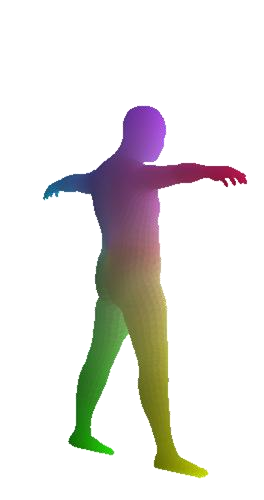
\includegraphics[width=0.45\linewidth]{human_object_coordinates}
    	\caption{The object coordinate representation of a human. Image taken from \cite{tsharp}.}
    	\label{fig:human_object_coordinates}
	\end{subfigure}
	\begin{subfigure}[t]{0.3\textwidth}
		\centering
    	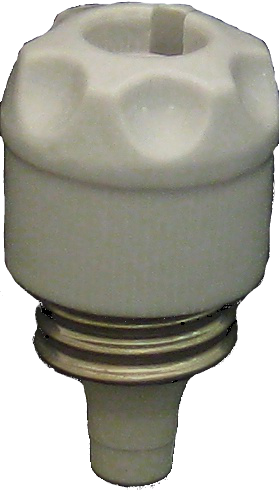
\includegraphics[width=0.45\linewidth]{tless_object}
    	\caption{An example object from the T-Less dataset. Image taken from \cite{tless}.}
    	\label{fig:tless_object}
	\end{subfigure}
	\begin{subfigure}[t]{0.3\textwidth}
		\centering
    	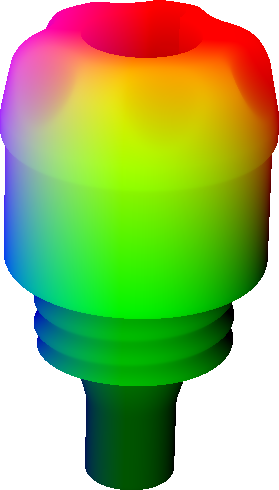
\includegraphics[width=0.45\linewidth]{tless_object_coordinates}
    	\caption{And the corresponding rendered 3D object coordinates (scaled for visualization). Own image.}
    	\label{fig:tless_object_coordinates}
	\end{subfigure}
	\caption{Example 3D coordinate representations.}
\end{figure} 

\textit{6D pose estimation} is a central task in the computer vision community. The goal is to retrieve an object's translation and rotation from an image, relative to the camera. \textit{6}D refers to the \textit{6-Degrees-of-Freedom (6-DOF)}, i.e. the 6 free parameters of the \textit{3}D translation and \textit{3}D rotation. The field of application ranges from medical imaging, robotics, augmented reality, and many others. Different systems provide different accuracy. Setups using two cameras for stereo vision or depth information in addition to colors achieve good results. As endoscopes usually do not provide depth information or stereo vision, this work focuses on pose estimation using RGB-only images. 

Early approaches extracted sparse features from the image and matched them against a large database to retrieve the pose. The accuracy of those methods suffers when objects are texture-less or poor-textured. Template-based methods rely mainly on the object's shape and therefore still work well on texture-less objects. Unfortunately, deformation of the object or partial occlusion is not handled well by templates and accuracy decreases significantly.

Deep learning enabled researchers to avoid manually modeling the features that are to be matched and instead make the systems learn the objects' appearances. There are different possible ways to estimate the pose with learning-based approaches. The 6 parameters can be predicted directly or an intermediate representation can be used for pose computation. Predicting the parameters directly can be problematic, as the output of the neural network underlies noise and there is no possibility to verify or improve the pose afterwards. This is the reason why this work employs a network with a dense output, i.e. one output  for each pixel. The output for a pixel are the 3D coordinates on the object. Each subset of object coordinates leads to a certain pose. Some coordinates may contradict a pose and therefore the pose with the least contradictions is chosen as the best one. The next section will introduce this concept of so-called object coordinates in depth.

\subsection{Object Coordinate Regression} \label{objectcoordinates}

\begin{figure}[!tbp]
	\centering
    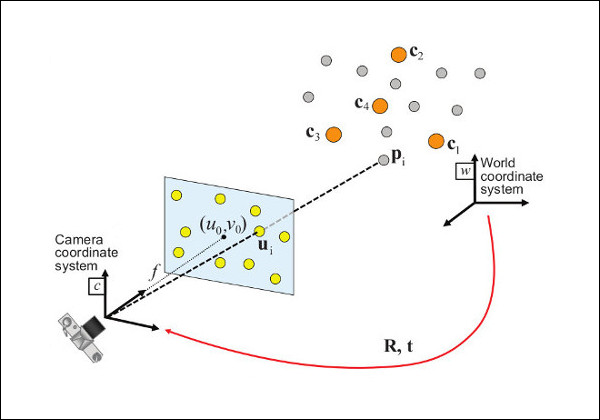
\includegraphics[width=0.45\linewidth]{pnp}
    \caption{The relationship between the camera, the 3D points and their projections on the screen using the rotation matrix $R$ and the translation vector $t$. Image taken from \cite{opencv_pnp}.}
    	\label{fig:pnp}
\end{figure} 

Tayler et al. first used object coordinates in \cite{tsharp}. Instead of directly predicting the location of joints or limbs of the human body they computed for each pixel the corresponding 3D location on the person (see fig. \ref{fig:human_object_coordinates}). The idea can be transfered to objects of any kind. Fig. \ref{fig:tless_object} shows an example object from the T-Less dataset \cite{tless} and fig. \ref{fig:tless_object_coordinates} shows the corresponding rendered 3D object coordinates.

The 3D coordinates and the respective 2D pixel locations on the image yield the \textit{Perspective-n-Point (PnP) Problem}. That is, for a given pixel $p$ on the image and the corresponding 3D point $x$ (both in homogeneous coordinates), a pose consisting of the rotation matrix $R$ and the translation vector $t$ has to fulfill the following equation

\begin{align}
 p = K \ [ \ R \ | \ t \ ] \ x \label{eq:pose_projection}
\end{align} 

where $K$ is the camera matrix

\begin{align}
K = \begin{bmatrix}
f_x & s & c_x \\
0 & f_y & c_y \\
0 & 0 & 1 
\end{bmatrix}
\end{align}

which projects the 3D point transformed into the camera coordinate system on the 2D image plane. $s$ is a skew factor which is usually $0$, $(c_x, c_y)$ is the principal point, usually the center of the image and $f_x$ and $f_y$ is the focal lengths in $x$ and $y$ direction respectively. The values for those variables can vary when for example cropping the image. Fig. \ref{fig:pnp} visualizes the relation of pixels and object coordinates. If equation \ref{eq:pose_projection} is overdetermined because there are more correspondences than variables it cannot be solved directly.

A common method to solve the PnP problem for many correspondences is to use the \textit{RANSAC algorithm} \cite{ransac}. RANSAC selects a model based on a subset of the dataset and evaluates it against the remaining data. This way the approximate best model is found iteratively. Algorithm \ref{algorithm:ransac} shows the outline of the RANSAC algorithm for pose estimation. The energy function can be varied. It can for example be the number of inliers. Inliers are 3D points whose reprojected 2D location is within a certain area of the actual 2D location. Since RANSAC is well known and employed in many different applications to estimate a model that fits a dataset best, we use it in this work to compute the pose. The implementation that is used is the one incorporated into the \textit{solvePnPRansac} method of the \textit{OpenCV} \cite{opencv} framework. 

\begin{algorithm}
\caption{RANSAC} \label{algorithm:ransac}
\begin{algorithmic} 
\REQUIRE Set of 3D points
\REQUIRE Set of corresponding 2D points
\REQUIRE Number of iterations $i$
\REQUIRE An energy function to score the pose hypothesis $E$
\STATE Set current energy $e=0$
\STATE Set current best pose hypothesis $h$ to $null$
\FOR{$1 ... i$}
\STATE Select a subset of corresponding points to compute pose $H$
\STATE Compute energy of the pose $e'=E(H)$
\IF{$e' > e$}
\STATE Store pose $H$ as current best in $h$
\STATE Set $e = e'$
\ENDIF
\ENDFOR
\RETURN Best pose $h$
\end{algorithmic}
\end{algorithm}